\documentclass{article}

\usepackage{pgf}
\usepackage{tikz}
\usetikzlibrary{arrows,automata}
\usepackage[latin1]{inputenc}
\begin{document}
	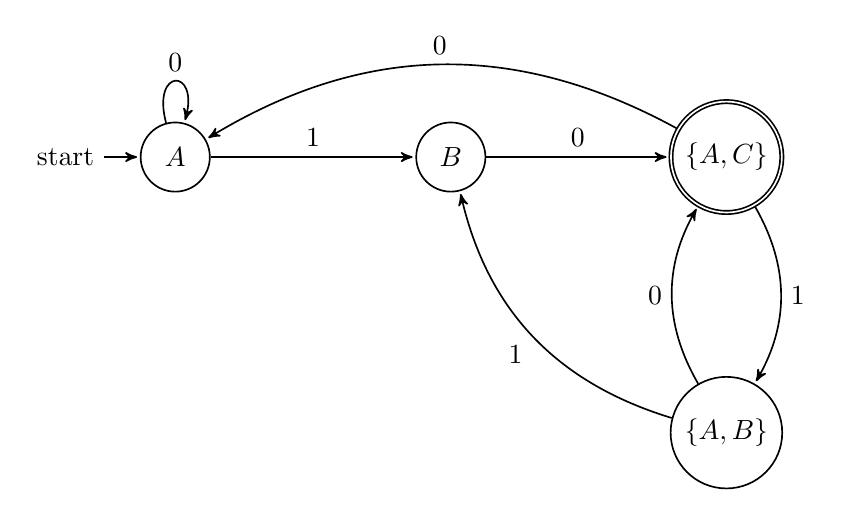
\begin{tikzpicture}[->,>=stealth',shorten >=1pt,auto,node distance=3.5cm,
	semithick]
	\tikzstyle{every state}=[fill=none,draw=#1,text=black]
	
	\node[initial,state]                 (A)                    {$A$};
	\node[state]                          (B) [right of=A] {$B$};
	\node[state, accepting]         (C) [right of=B] {$\{A,C\}$};
	\node[state]                          (D) [below of=C] {$\{A,B\}$};
	
	\path (A) edge                  node {1} (B)
	edge [loop above]  node {0} (B)
	(B) edge                     node {0} (C)
	(C) edge [bend right, above] node {0} (A)
	edge [bend left]   node {1} (D)
	(D) edge [bend left]   node {0} (C)
	edge [bend left]   node {1} (B);
	
	\end{tikzpicture}
	
\end{document}